\chapter{Background} \label{chap:background}

\section*{}

\minitoc \mtcskip \noindent
This chapter describes the necessary foundations regarding the Internet-of-Things context. \sectionintroref{sec:background_iot} describes the background of the Internet-of-Things paradigm and important concepts in that area, with a description of IoT architectures, including Fog and Edge, in \sectionintroref{sec:architectures}. Finally, \sectionintroref{sec:background_vpl} mentions visual programming languages, their uses as well as their benefits and drawbacks.

\section{Internet-of-Things}\label{sec:background_iot}

The Internet-of-Things paradigm is defined by the committee of the International Organization for Standardization and the International Electrotechnical Commission~\cite{ISOIEC} as:

\begin{quote}
    \emph{"An infrastructure of interconnected objects, people, systems and information resources together with intelligent services to allow them to process information of the physical and the virtual world and react."}
\end{quote}

\noindent
IoT systems are, mostly, networks of heterogeneous devices attempting to bridge the gap between people and their surroundings. According to Buuya~\cite{iot_future_direction}, the applications of IoT systems can be divided into four categories: (i)~\textit{Home}, at the scale of a few individuals or domestic scenarios, (ii)~\textit{Enterprise}, at the scale of a community or larger environments, (iii)~\textit{Utilities}, at a national or regional scale and (iv)~\textit{Mobile}, which is spread across domains due to its large scale in connectivity and scale. 

One might think that IoT only relates to machines and interactions between them. Most of the devices we use in our day-to-day --- \emph{e.g.}, mobile phones, security cameras, watches, coffee machines --- are computation capable of making moderately complex tasks and are continually generating and sending information. This incrementally translates towards the \emph{human-in-the-loop} concept, where humans and machines become part of a "symbiotic" relationship~\cite{human_in_the_loop_survey}.
 
\subsection{IoT architectures}\label{sec:architectures}

Internet-of-Things systems deal with big amounts of data from different sources and have to process it in an efficient and fast fashion~\cite{lin_survey}. Typical IoT systems are composed of three tiers~\cite{Yang2019}, which are:

\begin{description}
    \item[Cloud Tier] mostly composed of data centers and servers, normally running remotely. It is characterized by having high computation power and latency.
    \item[Fog Tier] composed of gateways and devices that are normally between the cloud servers and the edge devices. This tier has less latency than the cloud, more heterogeneity, and, typically, is more geographically distributed.
    \item[Edge Tier] composed of all the peripheral devices (\emph{e.g.}, sensors, embedded systems, light sources and air conditioners). These devices have several limitations in computational capabilities, but exhibit less latency since the data is processed in the same place it is captured.
\end{description}

Complementary to these tiers, we can also partition IoT systems into an Application Layer, a Network Layer, and a Perception Layer~\cite{iot_layers}. At first sight, these might seem compatible with the tiers mentioned above (in the same order); however, not all devices in each tier map to their respective layer. One example is a third-party service that provides readings, \eg Application Programming Interface (API) that provide temperature readings. It can be contained in the Perceptive Layer, but it is not included in the Edge Tier.

New paradigms of computing emerged related to each of these tiers. The majority of IoT systems use a Cloud Computing architecture~\cite{cisco}, taking advantage of centralized computing and storage. This approach poses some benefits, such as increased computational capabilities and storage, as well as easier maintenance. However, it also comes with several shortcomings such as (1)~higher latency, and~(2) higher usage of bandwidth, due to the need to send the data generated from the sensors back to the centralized unit(s)~\cite{connecting_fog_and_cloud}. Systems that only use cloud computing face several challenges~\cite{aazam2014cloud}, especially in real-time applications, which are sensitive to increased latency~\cite{latency_critical,EUC2018}. But with the increasing computation capabilities of edge devices and the requirement of reduced latency, two new paradigms appeared: Fog Computing and Edge Computing.

\subsubsection{Fog Computing}\label{sec:fog_computing}

The improvement of wireless technologies and the increasing computational power and reduced costs of lower-tier devices (\emph{i.e.}, fog and edge) allow the usage of these devices as computational resources in IoT systems. By not depending so much on the cloud tier, communication and resource sharing between devices can occur with lower latency and reduced amount of data transferred to the central instance. The central coordinator (on-premises or cloud-based), which in Cloud Computing was responsible for all the computation, now serves as an orchestrator of the communication between devices, occasionally providing necessary resources. This paradigm is called Fog Computing, where fog and edge devices are leveraged as computational entities, instead of merely sensors, actuators and gateways. It focuses on distributing data throughout the IoT system, from the cloud to the edge devices, making the system distributed and bringing computation closer to the perception tier~\cite{mobile_cloud}.

According to Buuya~\cite{IoT_principles_and_paradigms}, Fog Computing poses several advantages: (1)~reduction of network traffic by having edge devices filtering and analyzing the data generated and sending data to the cloud only if necessary, (2)~reduced communication distance by having the devices communicate between them without using the cloud as a middleman, (3)~low-latency by moving the processing closer to the data source rather than communicating all the data to the cloud for it to be processed, and (4)~scalability by reducing the burden on the cloud, which could be a bottleneck for the system.

\begin{figure}[h]
\centering
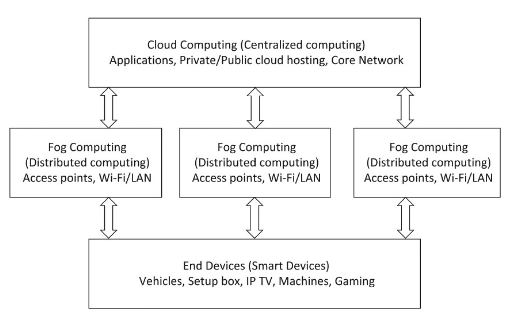
\includegraphics[width=0.8\textwidth]{fog_computing_architecture.png}
\caption[Fog Computing Architecture]{Fog Computing Architecture~\cite{IoT_principles_and_paradigms}}
\label{fig:fog_architecture}
\end{figure}

Despite all the advantages, Fog Computing has several challenges and difficulties. One of them is the management of resources and service allocation, responsible for deciding which tasks will be performed in the fog and where in the fog they will be allocated ~\cite{mukherjee}. The complexity is also more significant than Cloud Computing since it needs to work with heterogeneous devices with different capabilities.
       
\subsubsection{Edge Computing}\label{sec:edge_computing}

Edge Computing, also known as Mist Computing, is a distributed architecture that uses the devices' computational power to process the data they collect or generate. It takes advantage of the Edge tier, which contains the devices closer to the end-user, such as smartphones, TVs and sensors. The goal of this paradigm is to minimize the bandwidth and time response of IoT systems while leveraging the computational power of the devices in them. It reduces bandwidth usage by processing data instead of sending it to the cloud to be processed, which is also correlated to reduced latency since it does not wait for the server response. In addition to these advantages, and related to their cause, Edge Computing also prevents sensitive data from leaving the network, reducing data leakage and increasing security and privacy~\cite{edge_computing, edge_computing_2019}.

In this paradigm, each device serves both as a data producer and a data consumer. Since each device is constrained in terms of resources, this brings several challenges such as system reliability and energy constraints due to short battery life. Other issues consist of the lack of easy-to-use tools and frameworks to build cloud-edge systems, non-existent standards regarding the naming of edge devices and the lack of security edge devices have against outside threats such as hackers~\cite{promise_of_edge_computing}.

There is some confusion in the research community regarding the concepts of Fog and Edge computing. The publication from Iorga et al.~\cite{fog_edge_differences} was used to inspire the definitions of these terms. Edge Computing focuses on executing applications in constrained devices, without worrying about storage or state preservation. On the other hand, Fog Computing is hierarchical and includes devices with more capabilities, capable of control activities, storage, and orchestration.

\subsection{IoT development tools}\label{sec:iot_tools}

There are several tools that allow the development of IoT systems, with some of them being specific to certain domains and use-cases. \sectionref{sec:home_assistant} presents and IoT development tool focused on the home automation domain, where \sectionref{sec:device_hive} presents a more generic tool.

\subsubsection{Home Assistant}\label{sec:home_assistant}

Home Assistant~\cite{home_assistant} is an open-source home automation system that supports several mainstream IoT devices such as ESPs, Amazon Alexa, Google Assistant, and others. The configuration of the system is made with the use of a \textit{.yaml} file that is loaded by the system when it starts. This configuration file contains the integrations to be made and their respective configurations.

After creating the system, the user can interact with it by using a progressive web application. The interface, which consists of a dashboard, can be modified by the user to match its needs, with the addition of new panels or even the creation of new elements. It has integration with their Lovelace~\footnote{https://github.com/home-assistant/frontend/} front-end and React~\footnote{https://reactjs.org/}. An example of a Home Assistant dashboard can be seen in \figureref{fig:home_assistant}. 

\begin{figure}[h]
\centering
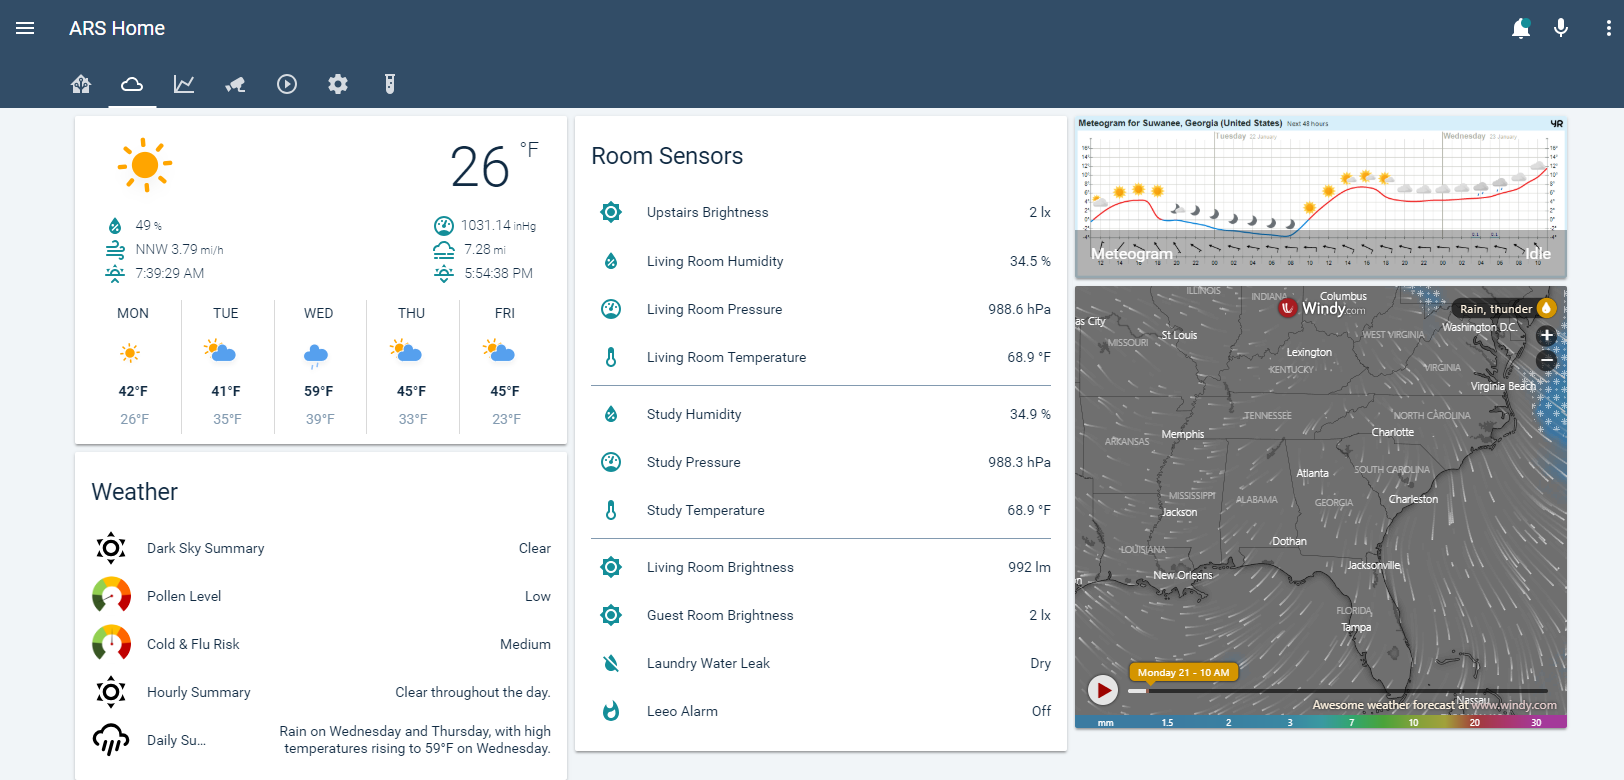
\includegraphics[width=1\textwidth]{home_assistant.png}
\caption[Example of a Home Assistant dashboard]{Example of a Home Assistant dashboard~\cite{homeassistant_image}}
\label{fig:home_assistant}
\end{figure}

The backend is made using Python3 and is composed of three modules: (1) the Home Control, responsible for collecting information and controlling the devices, (2) the Home Automation, responsible for triggering commands based on the user configuration, and (3) the Smart Home, for triggering commands based on previous interactions.

\subsubsection{Device Hive}\label{sec:device_hive}

Device Hive~\cite{device_hive} is an open-source IoT platform that supports multi-platform libraries for the development of IoT system in several domains (\eg home automation, smart energy, monitoring, remote control and others). It integrates with different types of devices, allowing modularity not only in the construction of client applications but also in the interfaces that connect with the devices. Device Hive is composed of three components: (1) the Auth service, responsible for the authorization and authentication of users and plugins, (2) the WebSocket Kafka Proxy, responsible for establishing communication between devices as well as allowing users to interact with plugins, and (3) the Plugin Management Service, that provides information about plugins, allows operations upon them and also allows the management of device operations.

Although the main core of the tool is a server that deals with all the devices and their data, it provides modules that can be integrated into the tool. They provide an Admin panel, which allows users to visually manage the connected devices and the installed plugins. It also integrates with Grafana~\footnote{https://grafana.com/} for data visualization. 

\section{Visual Programming Languages}\label{sec:background_vpl}

Having seen the characteristics and different ties of IoT, we will now address one of the most user-friendly ways of developing IoT systems.

Visual Programming, as defined by Shu~\cite{vpl_definition_shu}, consists of using meaningful graphical representations in the process of programming. We can consider Visual Programming Languages (VPLs) as a way of handling visual information and interaction with it, allowing the use of visual expressions for programming. According to Burnet and Baker~\cite{scaling_vpls}, visual programming languages are constructed to \emph{ "improve the programmer's ability to express program logic and to understand how the program works"}. There are several applications of visual programming languages in different areas, such as education, video game development, automation, multimedia, data warehousing, system management, and simulation, with this last area being the one with the most use cases~\cite{survey_vpl_iot}.

Visual programming languages exhibit several characteristics, such as a concrete and visual process and depiction of the program, immediate visual feedback, and usually require less knowledge of programming concepts~\cite{scaling_vpls}. VPLs can be categorized~\cite{vpls_survey} in the following way: 
\begin{description}
    \item[Purely Visual Languages], where the system is developed using only graphical elements and the subsequently debugging and execution is made in the same environment;
    \item[Hybrid text and visual systems], where the programs are created using graphical elements, but their execution is translated into a text language;
    \item[Programming-by-example systems], where a user uses graphical elements to teach the system;
    \item[Constraint-oriented systems], where the user translates physical entities into virtual objects and applies constraints to them, in order to simulate their behaviour in reality;
    \item[Form-based systems], which are based on the architecture and behaviour of spreadsheets.
\end{description}

Some of these categories can be simultaneously present in a single system, making them not mutually exclusive.

\subsection{Node-RED}\label{sec:node-red}

Node-RED~\cite{node_red} is a visual programming tool applied to the development of Internet-of-Things systems. It was first developed to manipulate and visualize mappings between Message Queuing Telemetry Transport (MQTT) topics in IBM's Emerging Technology Services group. It then expanded into a more general open-source tool, which is now part of the JS Foundation.

It is a web-based tool consisting of a run time built with the Node.js framework and a browser-based visual editor. This tool provides the end-user with a simple interface to connected devices and APIs, using a flow-programming approach~\cite{node_red}. Programs are called \emph{flows}, built with \emph{nodes} connected by wires. Each node corresponds to an action, such as input, output, data processing, etc.

The Node-RED interface has three components: (1)~Palette, (2)~Workspace and (3)~Sidebar. The Palette contains all the nodes installed and available to use, divided into categories. They can be used by dragging them into the workspace and additional features for each node are accessible by double-clicking them. The Workspace is where the flows are created and modified. It is possible to have several \emph{flows} and \emph{sub-flows} accessible with the use of tabs. Lastly, the Sidebar contains information about the nodes, the debug console, node configuration manager and the context data. \figureref{fig:node_red_window} showcases the visual interface of Node-RED and its elements.

\begin{figure}[h]
\centering
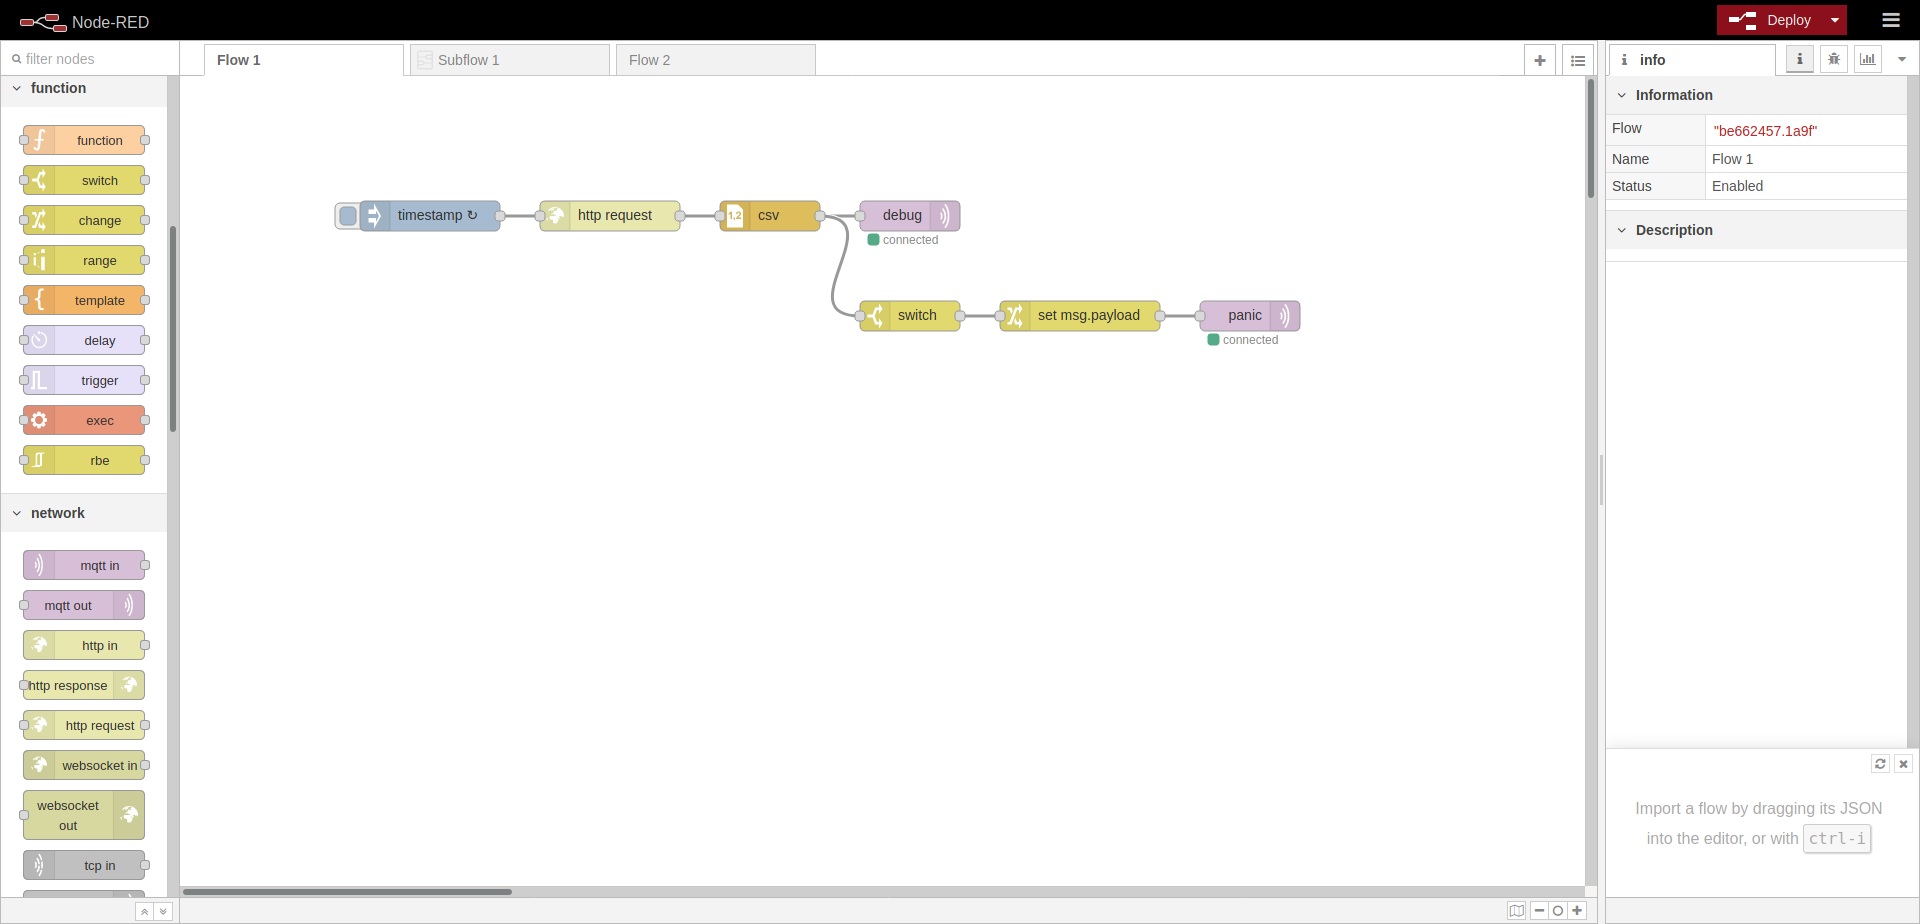
\includegraphics[width=1\textwidth]{node_red_window.png}
\caption{Node-RED environment}
\label{fig:node_red_window}
\end{figure}

One example of a \emph{flow} can be seen in \figureref{fig:node_red_example}, where a request is being made in intervals of 5 minutes to an HTTP URL that returns a CSV with the feed of significant earthquakes in the last 7 days. The data from the CSV is then printed to a MQTT topic and, if the magnitude is equal or bigger than 7, the message "PANIC!" is printed to other MQTT topic. 

\begin{figure}[!ht]
\centering
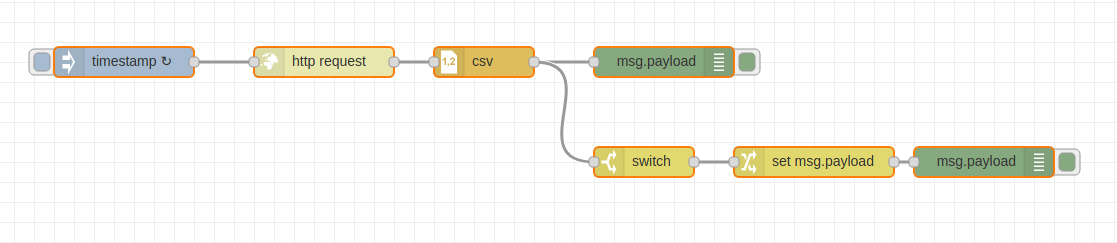
\includegraphics[width=1\textwidth]{node_red_example.png}
\caption{Example of a Node-RED flow}
\label{fig:node_red_example}
\end{figure}

Node-RED is modular, allowing the installation of community-made extensions, such as \textit{nodes}. These custom nodes extend from the base class \texttt{Node}, which implements an event based communication. Each node sends and receives messages, triggering events that execute each \textit{node}'s specific behaviour.

Being open-source, Node-RED takes advantage of a large community that contributes with new nodes and improvements to the tool. It is the most popular open-source visual programming tool for IoT, with more than 9,300 stars on Github.

\subsection{Godot}\label{sec:godot}

There are also other domains besides IoT where visual programming languages are being used. One example is the game engine Godot~\footnote{https://godotengine.org/} with its visual scripting. Godot is an open-source game engine that has recently increased in popularity, currently having 31,600 stars on GitHub~\footnote{https://github.com/godotengine/godot}. It offers several alternatives for its users to program their games, from using C++ to their own GDScript. However, to lower the barrier for a user to start using the engine, allowing people with no programming experience to easily understand the flow of logic, they developed a visual alternative --- visual scripting \seefigureref{fig:godot}.

\begin{figure}[!ht]
\centering
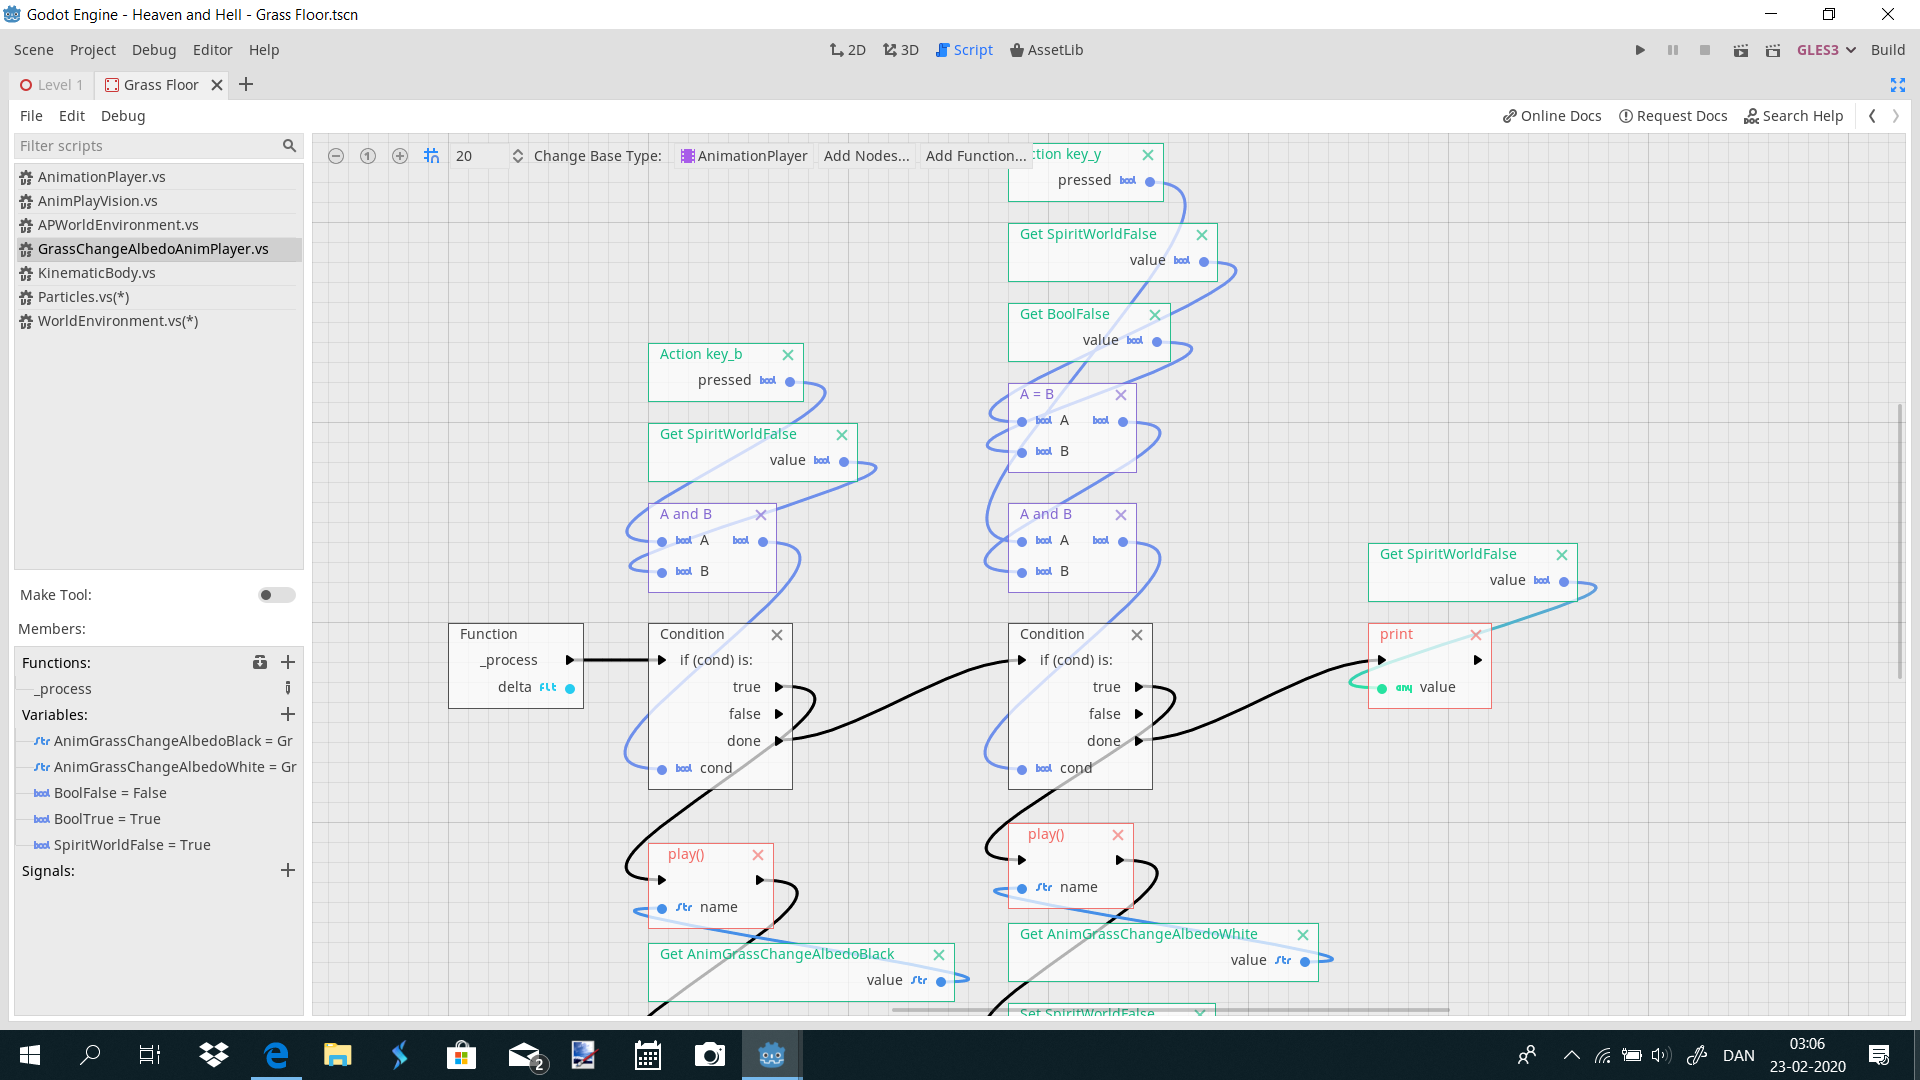
\includegraphics[width=1\textwidth]{godot_vpl.png}
\caption[Godot visual scripting]{Godot visual scripting~\cite{godot_image}}
\label{fig:godot}
\end{figure}

Each node corresponds to a function in a normal text script. Each node contains properties, ports and connections. Properties consist of arguments the function receives, as well as arguments globally accessible by the script. Ports and connections consist of inputs and outputs it can receive, either from other nodes or signals emitted during the events of the game.

Although most features are implemented in this visual alternative, it does not substitute programming with code, since visual scripting takes more time to develop code and it hinders project scalability.

\subsection{Blender}\label{sec:blender}

Blender~\footnote{https://www.blender.org/} is an open-source 3D creation suite that supports that entirety of the 3D pipeline. It is open to the community, with its source code being under the GPL license. It contains a visual programming editor, called Node Editor, which works with 3 types of nodes: (i) material, (ii) composite and (iii) texture nodes. \figureref{fig:blender} contains an example of a composition.

\begin{figure}[!ht]
\centering
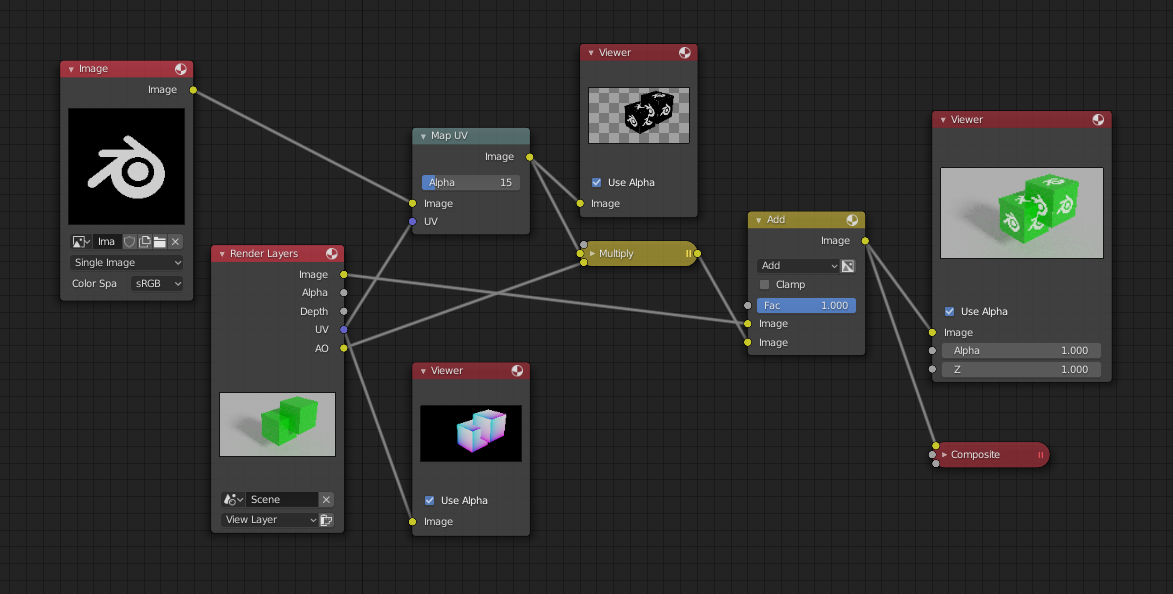
\includegraphics[width=1\textwidth]{blender_image.png}
\caption[Blender composition node editor]{Blender composition node editor~\cite{blender_image}}
\label{fig:blender}
\end{figure}

Each node contains a title, inputs, outputs, and properties. Properties are visible in each node and can be altered, which possible results in different outputs.The inputs and outputs are located at the bottom left and top right, respectively. 

\section{Decentralized Orchestration}\label{sec:background_decentralized_orchestration}

As mentioned in \sectionref{sec:architectures}, several IoT architectures focus on a more decentralized approach, allocating tasks in devices present in Fog and Edge tiers. This concept or decentralized orchestration is present in other domains besides IoT. One example of decentralized orchestration in Kubernetes~\footnote{https://kubernetes.io/}.

Kubernetes is an open-source system for automating deployment scaling and management of applications. It includes features such as load balancing, service discovery, self-healing and scaling. When Kubernetes is deployed, a \textit{cluster} is created. This \textit{cluster} contains \textit{nodes} that run containerized applications, which in turn can host \textit{pods}. Pods are processes that represent an instance of an application, which might translate into a single container or multiple tightly-coupled containers. They might have predicates, which are constraints that cannot be violated, and priorities, which would be beneficial if accomplished but can violated if not possible.

Each Kubernetes instance is composed of a scheduler, an API server, an etcd, a kube controller manager and a cloud controller manager~\cite{kubernetes_components}. The scheduler is responsible for assigning \textit{pods} to \textit{nodes}. The API exposes the Kubernetes API, allowing users to interact with the system. The etcd consists of a key-value store for storing all the \textit{cluster} data. The controllers deal with process specific management, \ie noticing if nodes become unavailable and maintaining the replication factor.

After the deployment of a Kubernetes instance, the scheduler assigns the \textit{pods} to \textit{nodes}. The operation consists of two steps: (i) filtering, where the available \textit{nodes} are filtered in order to not violate the \textit{pod}'s predicates, and (ii) scoring, where the scheduler uses the remaining \textit{nodes} from the filtering process and ranks them regarding their compliance to the \textit{pods} priorities~\cite{kubernetes_scheduler}. 

Finally, the scheduler assigns each \textit{pod} to the \textit{node} with the highest ranking. The filtering process might result in an impossible assignment, if there are no \textit{nodes} that comply with a \textit{pod}'s predicates. 

\section{Summary}

This chapter introduces concepts regarding IoT, visual programming and decentralized orchestration, which are fundamental to the understanding of this dissertation. \sectionref{sec:background_iot} defines Internet-of-Things, as well as its use cases. Fog and Edge computing paradigms are explained, which will be mentioned throughout this document, as well as examples of tools for the development of IoT systems. \sectionref{sec:background_vpl} introduces and explains the definition and categorization of visual programming languages, with examples of their application in several domains. Finally, \sectionref{sec:background_decentralized_orchestration} exposes decentralized orchestration implementations such as Kubernetes.
